\documentclass[11pt,letterpaper]{article}
\usepackage[lmargin=1in,rmargin=1in,tmargin=1in,bmargin=1in]{geometry}
\usepackage{../style/homework}
\usepackage{../style/commands}
\setbool{quotetype}{true} % True: Side; False: Under
\setbool{hideans}{false} % Student: True; Instructor: False

% -------------------
% Content
% -------------------
\begin{document}

\homework{13: Due 04/26}{Might is geometry; joined with art, resistless.}{Euripides}

% Problem 1
\problem{10} Suppose that triangle $\Delta DEF$ is congruent to the triangle $\Delta ABC$, shown below. \par
	\[
	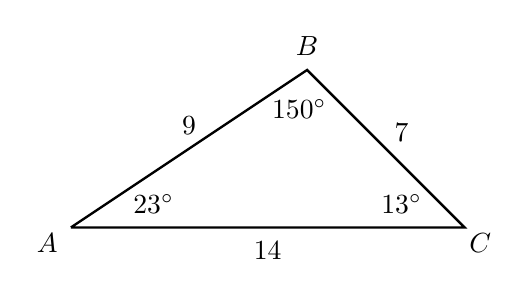
\begin{tikzpicture}
	\draw[line width=0.03cm] (0,0) -- (3,2) -- (5,0) -- (0,0);
	\node at (-0.3,-0.2) {$A$};
	\node at (3,2.3) {$B$};
	\node at (5.2,-0.2) {$C$};
	\node at (1.5,1.3) {$9$}; 
	\node at (4.2,1.2) {$7$}; 
	\node at (2.5,-0.3) {$14$}; 
	\node at (1.05,0.3) {$23^\circ$};
	\node at (4.2,0.3) {$13^\circ$};
	\node at (2.9,1.5) {$150^\circ$};
	\end{tikzpicture}
	\]
Find the following:
	\begin{enumerate}[(a)]
	\item $\angle FED$
	\item $|\overline{FD}|$
	\item $\angle EDF$
	\item $|\overline{DE}|$
	\item $\angle DFE$
	\item $|\overline{EF}|$
	\end{enumerate} \pspace

\sol 
\begin{enumerate}[(a)]
\item $\angle FED= 150^\circ$
\item $|\overline{FD}|= 14$
\item $\angle EDF= 23^\circ$
\item $|\overline{DE}|= 9$
\item $\angle DFE= 13^\circ$
\item $|\overline{EF}|= 7$
\end{enumerate}



\newpage



% Problem 2
\problem{10} Does there exist a triangle with sides 5, 6, 12? If not, explain why. If so, construct. Do the same for a triangle with sides 5, 12, 13. \pspace

\sol The sides of a triangle must obey the triangle inequality, i.e. for any sides $a$, $b$, $c$, of a triangle, we must have $a + b > c$. Furthermore, if given three positive numbers $a$, $b$, $c$, if any two of $a$, $b$, $c$ have sum greater than the other, then there exists a triangle with side lengths $a$, $b$, and $c$. \pspace

There does not exist a triangle with sides 5, 6, and 12 because $5 + 6= 11 < 12$, which would violate the triangle inequality. However, because $5 + 12= 17 > 13$, $5 + 13= 18 > 12$, and $12 + 13= 25 > 5$. 



\newpage



% Problem 3
\problem{10} A student is given a line segment $\overline{AB}$ and is told to construct the perpendicular bisector to the segment; that is, construct a line segment that is perpendicular to the given line segment that intersects the given line segment at a point $C$ such that $|\overline{AC}|= \overline{BC}|$. The student then performs the following:
	\begin{itemize}
	\item They draw a circle centered at $A$ with radius equal to the length of the line segment. 
	\item They draw another circle centered at $B$ with radius equal to the length of the line segment. 
	\item They find the two intersection points of the circles from the previous two steps and connect them.
	\end{itemize}
The student then claims that the final line segment drawn is the perpendicular bisector of the line segment $\overline{AB}$. Is the student correct? If so, prove that this is the perpendicular bisector. If not, explain what they have done incorrectly. \pspace

\sol Indeed, this construction yields the perpendicular bisector of the segment. One can easily verify that all `adjacent' triangles are congruent so that the segment splits the segment into two congruent parts and does so perpendicularly. 


\end{document}